\section{Dataset: rebuilding the corpus and measuring its quality}\label{sec:dataset}
We take the \emph{Dataset Research Track}: besides rebuilding the paper's corpus we release a
provenance-documented manifest with two deduplication levels, near-duplicate clusters and two additional
evaluation protocols (``GlareShell-R''; data card in \texttt{docs/DATA\_CARD.md}, schema in
\texttt{docs/SCHEMA.md}, label guide in \texttt{docs/LABEL\_GUIDE.md}).

\subsection{Sources and provenance}
We cloned every repository of the paper's Table~1 at pinned revisions (\Cref{tab:funnel}).
\texttt{ysrc/webshell-sample} has been deleted from GitHub; its files survive only inside the
Cyc1e183 aggregate~\cite{cyc1e183}, a ``cleaned'' set of 2,917 webshells drawn from 17 collections, which
dominates the webshell side. Its files are named by MD5 and carry no origin; matching MD5s against the
collections we could clone recovers the origin of only 646 of them (2,271 remain \emph{unknown}).
Benign files come from pinned releases (WordPress~6.4.3, Drupal~10.2.5, Laravel skeleton v10.3.3,
PHPMailer~6.9.1, doorGets CMS). For the dataset track we add four \emph{held-out} benign projects
(Laravel framework v10.48.4, phpMyAdmin~5.2.1, Joomla~5.0.3, Matomo~5.0.3) and two held-out webshell collections
(BlackArch, xl7dev). Licenses range from CC0/MIT to GPL; several webshell collections state none, which is
one more reason we never redistribute samples publicly (\Cref{sec:ethics}).

\begin{table*}[!t]
\centering\footnotesize
\caption{Corpus funnel per source. ``exact'' = first copy per SHA-256 (the paper's dedup); ``ws'' = first copy per
whitespace-insensitive hash. Duplicates are resolved in favour of the paper sources, so the small numbers for the
individual webshell collections mean that their files are already inside Cyc1e183.}
\label{tab:funnel}
\begin{tabular}{@{}lllrrrr@{}}
\toprule
Label & Subset & Source & PHP-ext files & contain \texttt{<?} & exact dedup & ws dedup \\ \midrule
benign & heldout & joomla/joomla-cms & 3105 & 3105 & 3104 & 3103 \\
benign & heldout & laravel/framework & 2193 & 2100 & 2100 & 2100 \\
benign & heldout & matomo-org/matomo & 3085 & 3071 & 2946 & 2946 \\
benign & heldout & phpmyadmin/phpmyadmin & 951 & 951 & 951 & 951 \\
benign & paper & PHPMailer/PHPMailer & 124 & 124 & 123 & 123 \\
benign & paper & WordPress/WordPress & 1452 & 1452 & 1448 & 1448 \\
benign & paper & doorgets/CMS & 1573 & 1568 & 1449 & 1443 \\
benign & paper & drupal/drupal & 9868 & 9866 & 9860 & 9860 \\
benign & paper & laravel/laravel & 51 & 50 & 50 & 50 \\
webshell & heldout & BlackArch/webshells & 201 & 186 & 15 & 1 \\
webshell & heldout & xl7dev/WebShell & 282 & 278 & 31 & 18 \\
webshell & paper & Cyc1e183/PHP-Webshell-Dataset & 2917 & 2908 & 2908 & 1645 \\
webshell & paper & JohnTroony/php-webshells & 119 & 110 & 27 & 3 \\
webshell & paper & bartblaze/PHP-backdoors & 184 & 181 & 33 & 10 \\
webshell & paper & tennc/webshell & 381 & 378 & 129 & 89 \\
\bottomrule
\end{tabular}

\end{table*}

\paragraph{Reproduced composition}
After exact-hash deduplication the paper sources yield \textbf{3,097 webshells} (paper: 3,104) and 12,930 benign
files. The paper reports 10,375 benign files without saying how they were chosen; we subsample proportionally per
project (seed 2024) to exactly that size. The webshell count matches the paper within 0.2\%, which suggests the
paper used \emph{exact-hash} deduplication.

\subsection{ICFG extraction statistics}
\Cref{tab:extraction} shows that extraction itself is \emph{label-dependent}: webshells are older, less
well-formed and much larger. 139 webshells (4.5\%) contain syntax errors that PHP-Parser recovers from, 477
(15.4\%) exceed the 2,000-statement cap (benign: 0.4\%), and 53 produce an empty graph. These are signals a
classifier can exploit without understanding behaviour (graph size), and failure modes that a real deployment must
handle (an unparsable upload is itself suspicious). Statement counts of webshells (\Cref{fig:stmtdist}) span four
orders of magnitude, as in the paper's Fig.~5. Extraction takes 11\,ms per file on average (P95 40\,ms) on one core.

\begin{table*}[!t]
\centering\footnotesize
\caption{ICFG extraction outcome (after the four extractor fixes of \Cref{sec:method}).}
\label{tab:extraction}
\begin{tabular}{@{}llrrrrrrrr@{}}
\toprule
Label & Subset & Files & Crash & Parse err. & Empty ICFG & Truncated & Median nodes & P90 nodes & ms/file \\ \midrule
benign & heldout & 9101 & 0 & 1 & 123 & 7 & 18 & 103 & 6.9 \\
benign & paper & 12930 & 0 & 1 & 590 & 49 & 14 & 99 & 7.9 \\
webshell & heldout & 46 & 0 & 7 & 3 & 4 & 25 & 755 & 26.6 \\
webshell & paper & 3097 & 4 & 139 & 53 & 477 & 11 & 875 & 36.6 \\
\bottomrule
\end{tabular}

\end{table*}

\begin{figure*}[!t]
\centering
\subfloat[Statements per webshell ICFG (cf.\ paper Fig.~5).\label{fig:stmtdist}]{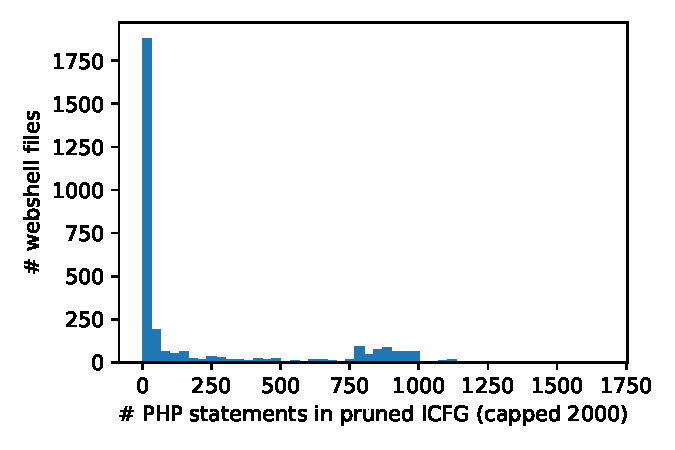
\includegraphics[width=0.42\linewidth]{figures/stmt_dist.pdf}}\hfil
\subfloat[Near-duplicate cluster sizes, paper webshells.\label{fig:clusters}]{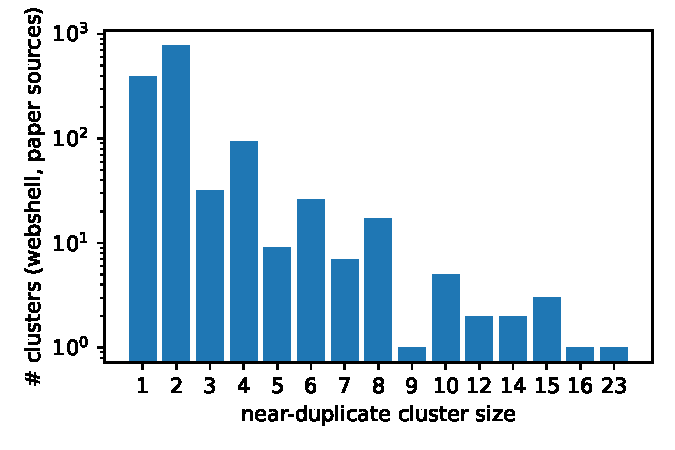
\includegraphics[width=0.42\linewidth]{figures/cluster_sizes.pdf}}
\caption{Corpus structure.}
\end{figure*}

\subsection{Near-duplicates and leakage}\label{sec:leak}
Exact hashing is a weak notion of ``unique'' for scripts that are copied, re-saved with different line endings,
re-branded or re-passworded. We measure duplication at two further levels:
\begin{itemize}
  \item \textbf{Whitespace-insensitive hash}: 1,265 of the 2,917 Cyc1e183 files (43\%) are byte-identical once
        whitespace is removed -- the ``cleaned'' dataset was deduplicated on raw bytes only.
  \item \textbf{Near-duplicate clusters}: we represent each file by the \emph{set} of its normalised ICFG statements,
        generate candidates with MinHash-LSH~\cite{broder1997minhash} (128 permutations, 32 bands) and merge pairs whose
        exact Jaccard similarity is $\ge 0.8$ (union-find). The 3,097 paper webshells collapse into \textbf{1,368
        clusters}; only 394 webshells are singletons and the largest family has 55 members (\Cref{fig:clusters}).
        Benign files are much less redundant (12,930 files $\rightarrow$ 11,828 clusters). No cluster mixes labels.
\end{itemize}
Under the paper's protocol (random 8:1:1), \textbf{77.0\% $\pm$ 4.4\% of test webshells have a near-duplicate in the
training set} (5 seeds; benign: 9.0\% $\pm$ 1.4\%). The paper's test set therefore mostly measures recognition of
already-seen families~\cite{allamanis2019duplication,arp2022dos}.

\subsection{Evaluation protocols}
\begin{description}
  \item[\pr] the paper's protocol: exact dedup, 3,097 webshells / 10,376 benign, stratified random 8:1:1.
  \item[\cg] leakage-controlled: whitespace dedup (1,747 webshells / 10,372 benign); whole near-duplicate clusters are
        assigned to train, validation or test (8:1:1 by file count, per label). Same sources as the paper.
  \item[\xs] generalisation: train/validation of \cg; test = held-out projects/collections after removing anything that
        shares a cluster with the paper sources: 9,091 benign files from four unseen projects and \textbf{only 18}
        unseen webshells. The latter is too small to estimate recall precisely (we give Wilson intervals); \xs{} is
        primarily a \emph{false-positive} stress test, which is the quantity that decides deployability.
\end{description}
Each protocol is instantiated with 5 seeds. We could not build a meaningful temporal split: git ``first-seen'' dates are upload dates, not
malware dates -- all 2,917 Cyc1e183 files share one commit (2020-11-13, a single zip), 98\% of xl7dev and 86\% of
BlackArch files share one day; only \texttt{tennc/webshell} has a spread history (100 distinct days, 2013--2023),
and its files are mostly already inside the aggregate. Source-disjointness (\xs) is our substitute.
